\section{Introduction}
%%% TODO: mention all figures in text 
%%% TODO: add motiviation for cell diffusion models from real world applications 
% from bridge paper:
Collective cell migration represents a fundamental process underpinning various biological phenomena, including embryonic development, tissue regeneration, wound healing, and the invasive potential of certain cancers. 
The collective nature of cell movement has been acknowledged for over a century, with early observations recognising its importance in developmental and regenerative processes~\cite{alert2020, holmes1914, herrick1932, vaughan1966}. 
However, the underlying mechanisms driving this coordinated behavior remained contentious, with competing hypotheses suggesting roles for pressure~\cite{herrick1932}, surface tension~\cite{alert2020}, or active forces generated by leading cells~\cite{holmes1914}. \\
Following a period where research emphasis shifted towards molecular and genetic details, the field has witnessed a resurgence of interest in understanding the physical principles governing collective cell migration. 
This revival is largely attributed to recent advances in experimental techniques~\cite{roca2017, du2005, trepat2009}, enabling direct measurements of mechanical forces exerted by cells, and the development of new conceptual frameworks in biophysics and active matter physics~\cite{marchetti2013, prost2015, julicher2018}, which challenged purely reductionist perspectives~\cite{good2018}. 
These developments coincided with a growing recognition of the critical role of collective cell migration not only in physiological processes but also in the progression of malignant diseases~\cite{friedl1995}. \\
The diverse manifestations of collective cell migration depend heavily on the specific biological context and tissue type~\cite{friedl2009}. 
For instance, epithelial cells often migrate as cohesive sheets on the extracellular matrix (ECM) during morphogenesis, wound closure, and regeneration. 
Snapshots from a cell wound healing process, illustrating the dynamics of cell migration, are shown in Figure~\ref{fig:woundhealing}. 

\begin{figure}[h!]
	\centering
	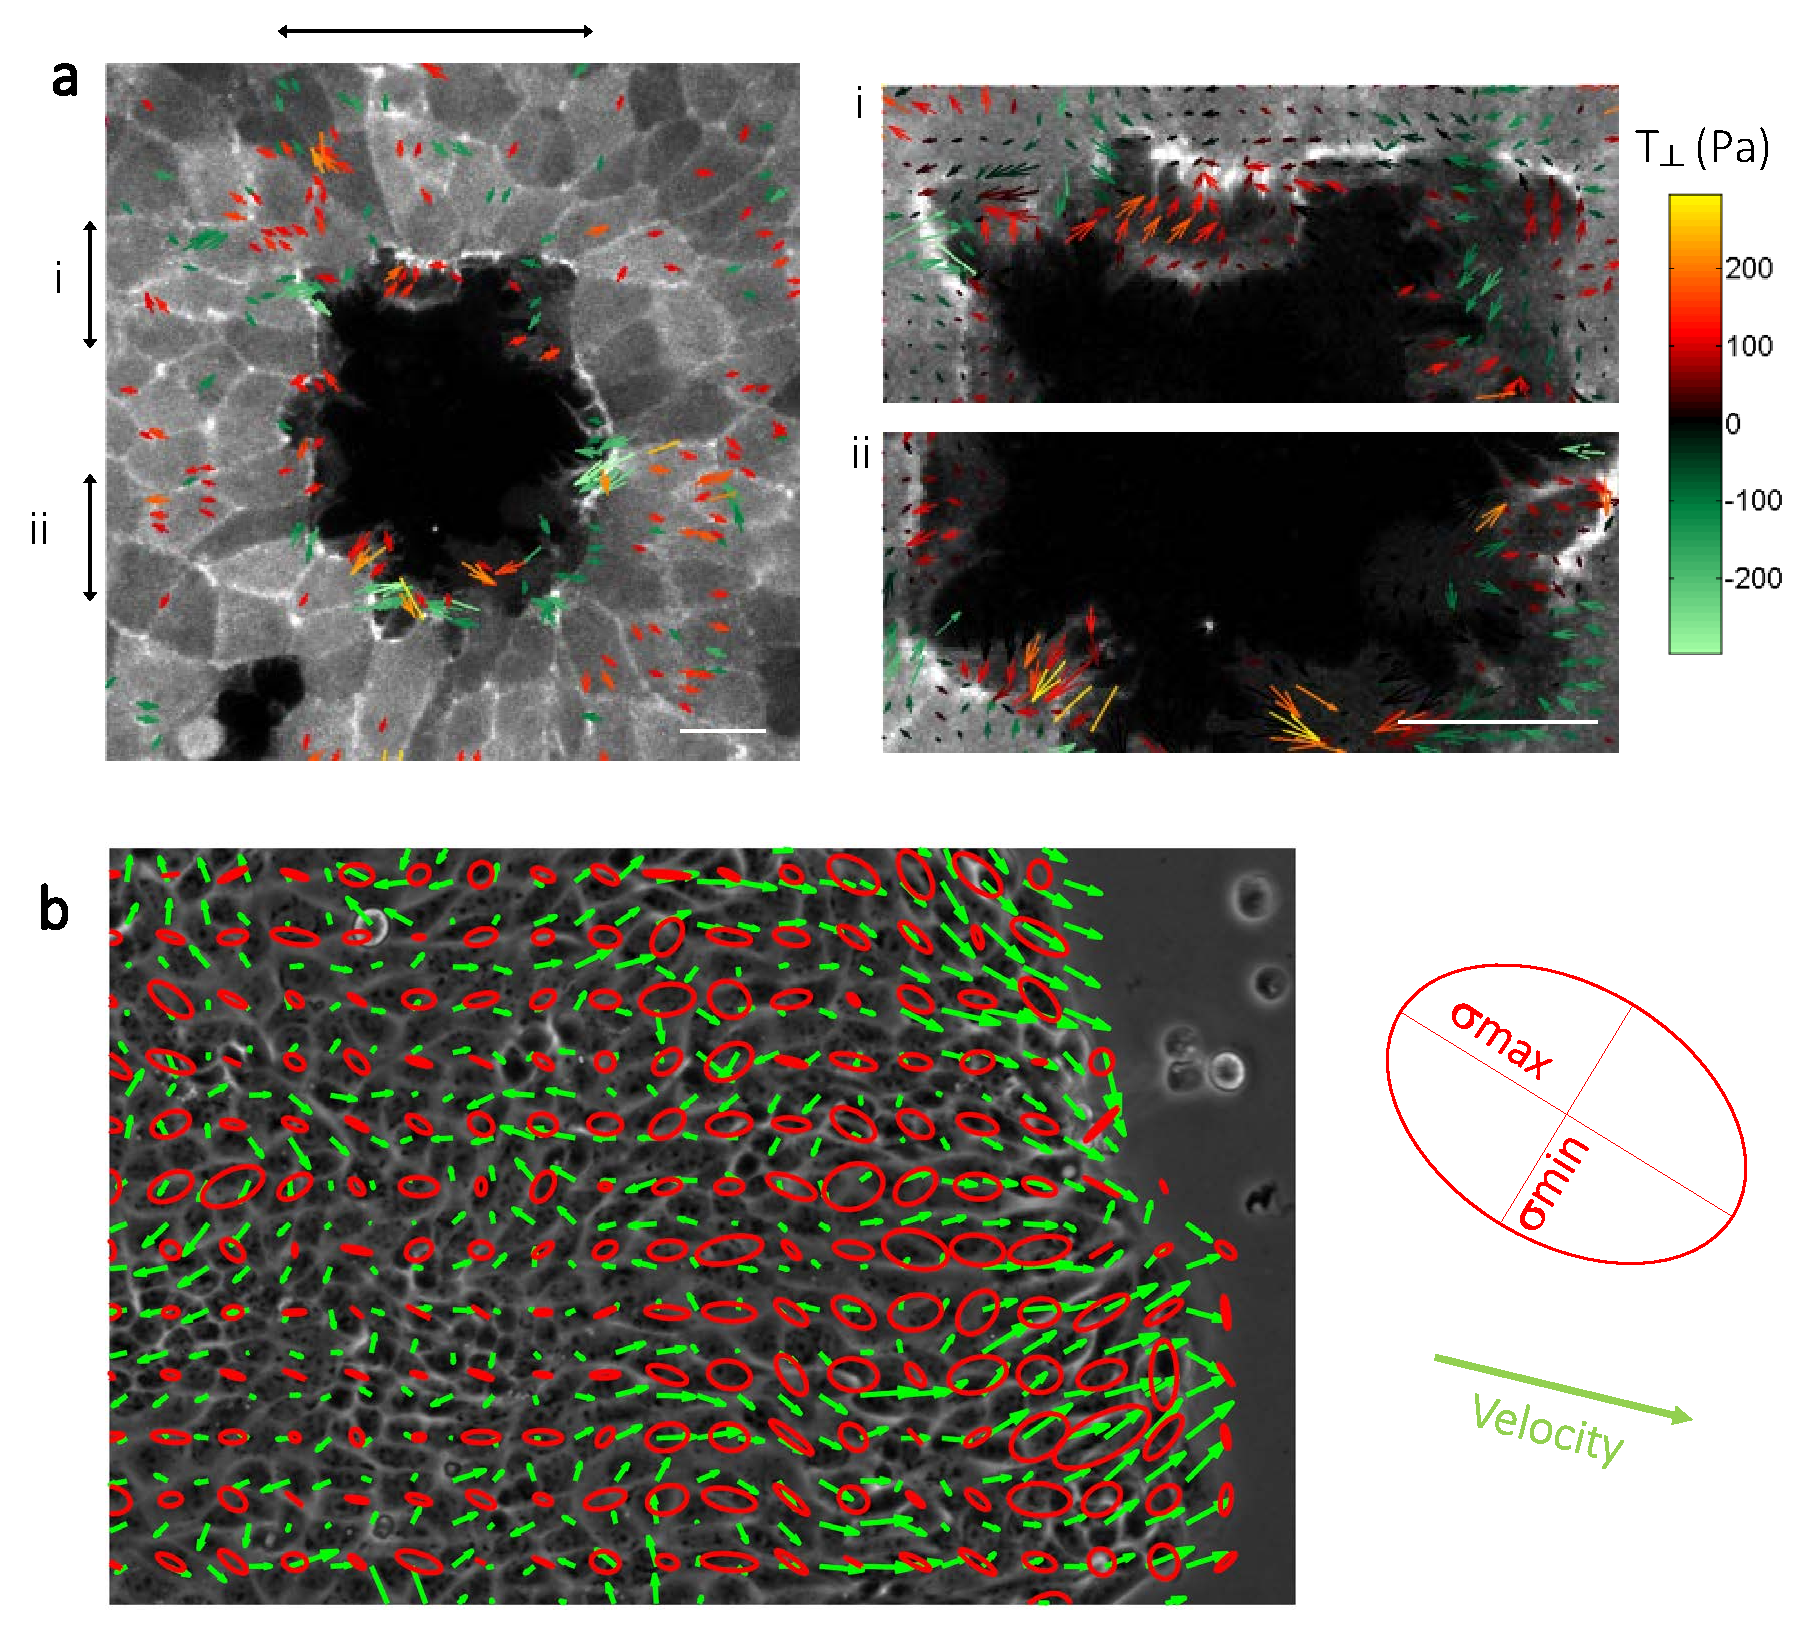
\includegraphics[width=0.8\textwidth]{intro/cell-migration.pdf}
	\caption{A figure from the paper~\cite{alert2020} illustrating cell migration during the wound healing process. 
	(a) Vector field representation of cellular traction forces in cells as they close a wound, with color intensity reflecting the radial component (positive values indicate outward-directed forces). 
	Panels labeled i and ii present magnified views of the regions marked by arrows in panel (a). 
	(b) Velocity vectors (green) and monolayer stress ellipses (red), depicting the principal stress directions and magnitudes, in a growing cell colony (phase contrast). 
	}
	\label{fig:woundhealing}
\end{figure}

In contrast, cancer cells often invade tissues as sheets, strands, or clusters, navigating a complex three-dimensional extracellular matrix (ECM) environment~\cite{friedl2009, cai2014, clark2015}. \\
While cell migration occurs extensively in three dimensions, modeling these complex processes remains a significant challenge. 
Consequently, much current scientific work focuses on two dimensional systems as a more tractable approach to understand the underlying physical principles.
Throughout this thesis, we consider cell dynamics within a bounded two-dimensional domain, denoted by $\Omega \subset \R^2$. 
Throughout this work, the total number of cells present within the domain $\Omega$ is denoted by $N_C \in \N$. \\
In two dimensions, cell monolayers serve as fundamental model systems to study cell behavior and tissue function. 
These systems, comprising a single layer of cells grown on a surface, can be mathematically and computationally modeled in either a confluent or non-confluent manner. 
A confluent cell model depicts a continuous, tightly packed layer where cells cover the entire surface without gaps, whereas a non-confluent monolayer represents a state with spaces and gaps between individual cells or cell clusters that have not yet achieved full surface coverage. \\
Recent years have seen growing interest in understanding the principles governing collective cell migration in confluent cell monolayers and epithelial tissues, which exhibit remarkable patterns and correlations in both structural arrangements and actively driven flows~\cite{wenzel2021}. 
Experimental studies on model systems have revealed phenomena such as unjamming transitions, spontaneous vortex formation, topological defects, and active turbulence. 
A key challenge is linking this macroscopic behavior to the properties of individual cells and their interactions, leading to a diverse range of modeling approaches spanning different levels of coarse-graining, from subcellular lattices and multiphase field models to vertex, Voronoi, particle, and continuum models. 
The systematic comparison of these diverse cell models is crucial for selecting appropriate methods for future studies and enabling predictive simulations of patterns and correlations in cell colonies. \\
Understanding the diffusion behavior of cells, influenced by various forces and interactions, is a key aspect of collective cell migration. This will be a central focus of this thesis. Different mathematical cell models, incorporating distinct cell dynamics, will exhibit varying diffusion behaviors. To begin this investigation, we will first introduce the simplest model: the point particle model. \\



\textbf{Point particle model} \\
We consider the point particle model on a two dimensional bounded domain $\Omega \subset \mathbb{R}^2$, where we have $N_C \in \N$ particles.
These particles have no real size.
There is also no particle interaction, as there is no possibility of collision. \\
Initially, the particles are randomly distributed in $\Omega$. \\
The particles' dynamics are governed solely by Brownian motion.
Brownian motion is a random and unpredictable motion that occurs in the real world when particles are suspended in a fluid and collide with surrounding molecules. \\
In mathematics, we model Brownian motion using stochastic differential equations (SDEs), which are equations that describe the motion of a particle over time in a random and unpredictable manner. 
SDEs are a powerful tool for modeling complex phenomena in physics, finance, and other fields, and are characterized by the presence of random terms that capture the uncertainty of the system. \\
Let 
\[\vec{x}_i(t) \in \Omega \quad 1 \leq i \leq N,\]
be the location of the particle $i$ at time $t > 0$. 
The particle movement can be modeled using the diffusion equation, which describes the random motion of particles over time
\begin{center}
	$d\vec{x}_i(t) = \sqrt{2D} \: dB_t^{(i)}, \quad 1 \leq i \leq N$,
\end{center}
where the constant $D > 0$ represents the diffusion coefficient which proportionally scales the speed of the particle movements by scaling the random fluctuations.
The term $dB_t^{(i)}$ introduces the randomness of Brownian motion, where $dB_t^{(i)}$ is a normally distributed random variable that accounts for the unpredictable changes in the position of particle $vec{x}_i$ over time. \\
We also consider the probability density function $\rho(t, \vec{x})$, which describes the probability of finding a particle at a specific position $\vec{x}$ at time $t$.
In the given context, the function $\rho$ satisfies the partial differential equation:
\begin{align}
	\dfrac{\partial \rho (t, \vec{x})}{\partial t} = D \Delta_{\vec{x}} \rho(t, \vec{x}) ,
	\label{equ:pointparticle}
\end{align}
where $\Delta_{\vec{x}}$ is the Laplacian operator with respect to the spatial variables. \\
Equation~\eqref{equ:pointparticle} represents the classic diffusion equation, a cornerstone of physics and mathematics.
The same diffusion constant $D>0$ is used in the SDE for particle movement and the PDE for the probability density function $\rho$. \\



% intro hp model 
\textbf{Hard sphere model} \\
Next, we consider models that add a real size to the particles and introduce particle interactions. 
With the inclusion of a real size, the particles cannot overlap, resulting in exclusion effects. 
To account for this, we introduce a new interaction dynamics that ensures the particles do not overlap. 
This new interaction dynamics leads to a more complex and realistic model that captures the behavior of particles with a real size and interactions. \\
Since particles cannot overlap, the domain $\Omega^{(i)}_{\epsilon}$, that holds the information where the centre of particle $i$ can be located, must exclude the areas where $\norm[\vec{x}_i - \vec{x}_j] \leq \epsilon$ for all $1 \leq j \leq N_C,$ $j \neq i$. 
This is due to the fact that particles cannot occupy the same space simultaneously. \\
The domain that holds all possible locations of the particles is then given by \[\Omega^{N_C}_{\epsilon} = \Omega^{(1)}_{\epsilon} \times \ldots \times \Omega^{(N_C)}_{\epsilon} .\] 
This can be visualized as a product space, where each particle's domain is combined to form a larger domain that encompasses all possible locations of the particles.
Under this circumstances, we will get a new dynamic compared to the point particle model.  
Figure~\ref{fig:hardsphere} illustrates how a hard sphere cell configuration looks like compared to a point particle configuration. \\

\begin{figure}[h!]
	\centering
	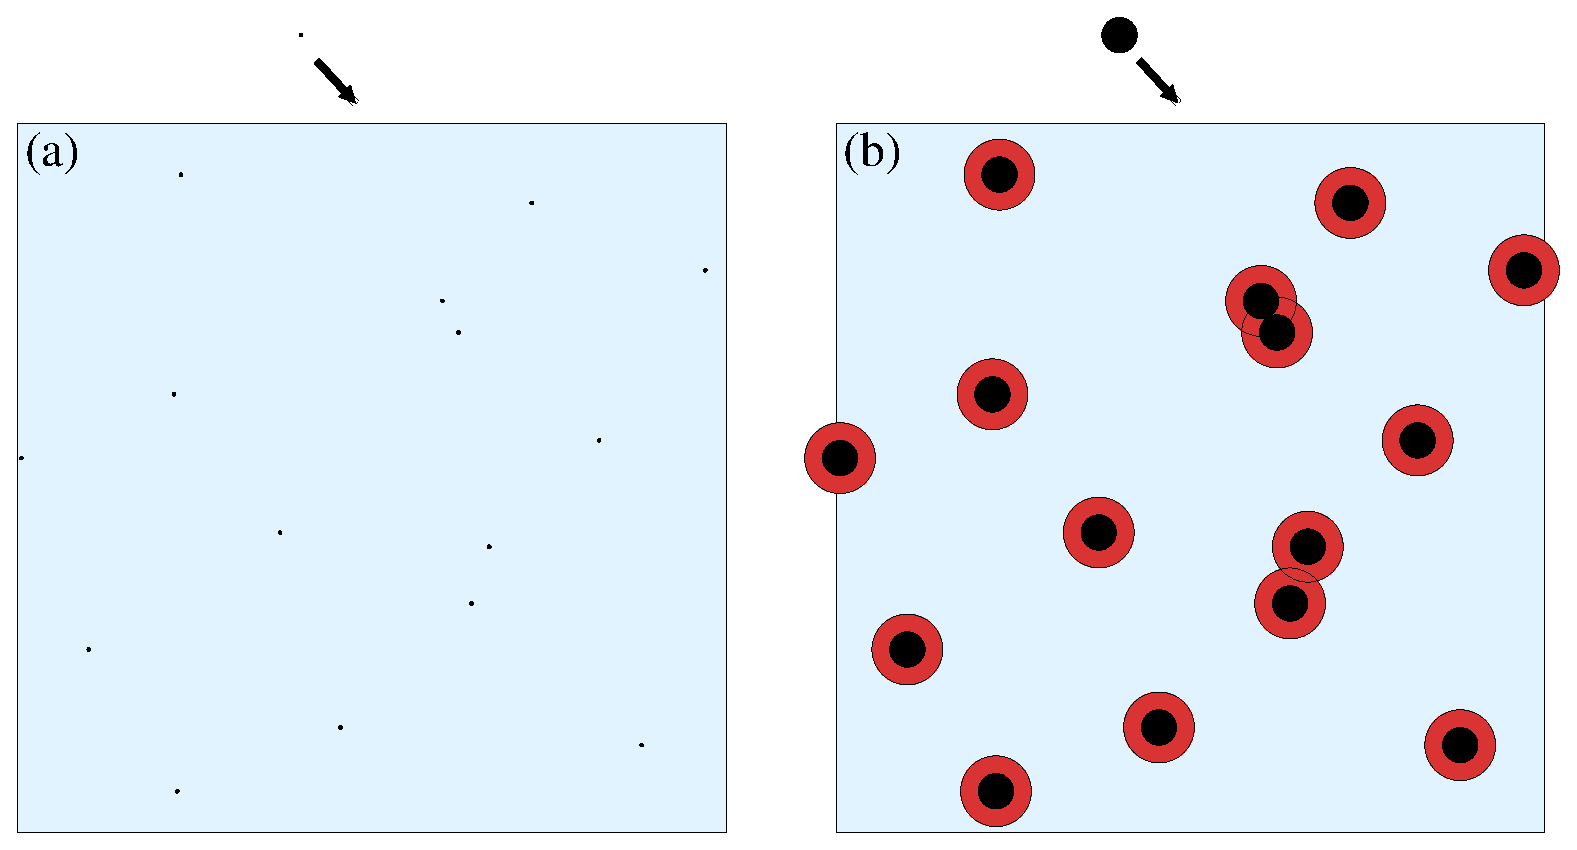
\includegraphics[width=0.8\textwidth]{intro/hardsphere.eps}
	\caption{An illustration from~\cite{Bruna2012} of the point particles on the left and the hard sphere particles on the right. We can see areas where the centre of the particles cannot be located, as they would overlap with other particles being marked red. 
	}
	\label{fig:hardsphere}
\end{figure}

In the work of Bruna et al.~\cite{Bruna2012}, a hard sphere particle model is examined.
Here, the particles are spherical in shape, with a diameter $0 < \epsilon \ll 1$.
All particles in this model are distinct and can be distinguished from one another. 
The diffusivity constant $D$ is set to be $D=1$. \\
The hard sphere model is characterized by the fact that any interaction between particles may cause a change in their direction of motion, but the spherical shape of the particles remains unchanged.
Hardcore collisions are modeled as reflective boundary conditions on the collision surfaces defined by $r = \norm[\vec{x}_i - \vec{x}_j] = \epsilon$, where $1 \leq i < j \leq N_C$.
The external forces acting on a particle in the system are described by the force function $f: \R^2 \rightarrow \R^2$, which depends only on the location of the particle.
The function $\vec{F}$ maps the particle configuration $\vec{X} = (\vec{x}_1, \ldots, \vec{x}_{N_C})^T$ to the vector of external forces $\vec{F}(\vec{X}) = (f(\vec{x}_1), \ldots, f(\vec{x}_{N_C}))^T$.
The dynamics of the particles are governed by the SDE
\begin{align*}
	d\vec{x}_i(t) = \sqrt{2D} \: dB_t^{(i)} + f(\vec{x}_i(t)) \: dt, \qquad 1 \leq i \leq N_C.
\end{align*}
In this model, the particles are initially randomly distributed in $\Omega^{N_C}_{\epsilon}$, ensuring that no overlap occurs between the particles.
The joint probability density function $P$ of the $N_C$ particles satisfies the high-dimensional Fokker-Planck equation
\begin{align*}
	\dfrac{\partial P}{\partial t} = \nabla_{\vec{X}} \cdot ( \nabla_{\vec{X}} P - P \vec{F}),
\end{align*}
where $\nabla_{\vec{X}}$ and $\nabla_{\vec{X}} \cdot$ denote the gradient and divergence operators with respect to the $N_C$-particle position vector $\vec{X}$.\\
Using the method of matched asymptotic expansions, the authors also derived the probability density function $\rho$ of finding a single particle at time $t$ and position $\vec{x}$, which satisfies the equation
\begin{align}
	\dfrac{\partial \rho (t, \vec{x})}{\partial t} = \Delta_{\vec{x}} \rho + \frac{\pi}{2} (N_C - 1) \epsilon^2 \Delta_{\vec{x}} (\rho^2) - \nabla_{\vec{x}} \cdot (f(\vec{x}) \rho).
	\label{equ:hardsphere}
\end{align}
When $f$ is neglected and $\epsilon \rightarrow 0$, this equation reduces to the probability density function of the point particle model, except for a rescaling factor.
The Fokker-Planck equation is a direct extension of the diffusion equation, with an additional drift term.\\
A central finding of~\cite{Bruna2012} is shown in Figure~\ref{fig:fig2BC12}, which compares the diffusion behavior of the point particle model and the hard sphere model. 
It uses the Monte Carlo method for the point particles and the hard sphere in order to give a numerical approximation of the density dynamic. 
The Monte Carlo method involves running the simulation many times ($M=10000$). 
For each discrete subsquare of our domain, we count how many particles were found at that location across all runs at time $t=0.05$. 
We then divide by the total number of runs to get the estimated probability density at that place and time. 
This estimated density converges to the true density as the number of runs increases. \\

\begin{figure}[h!]
	\centering
    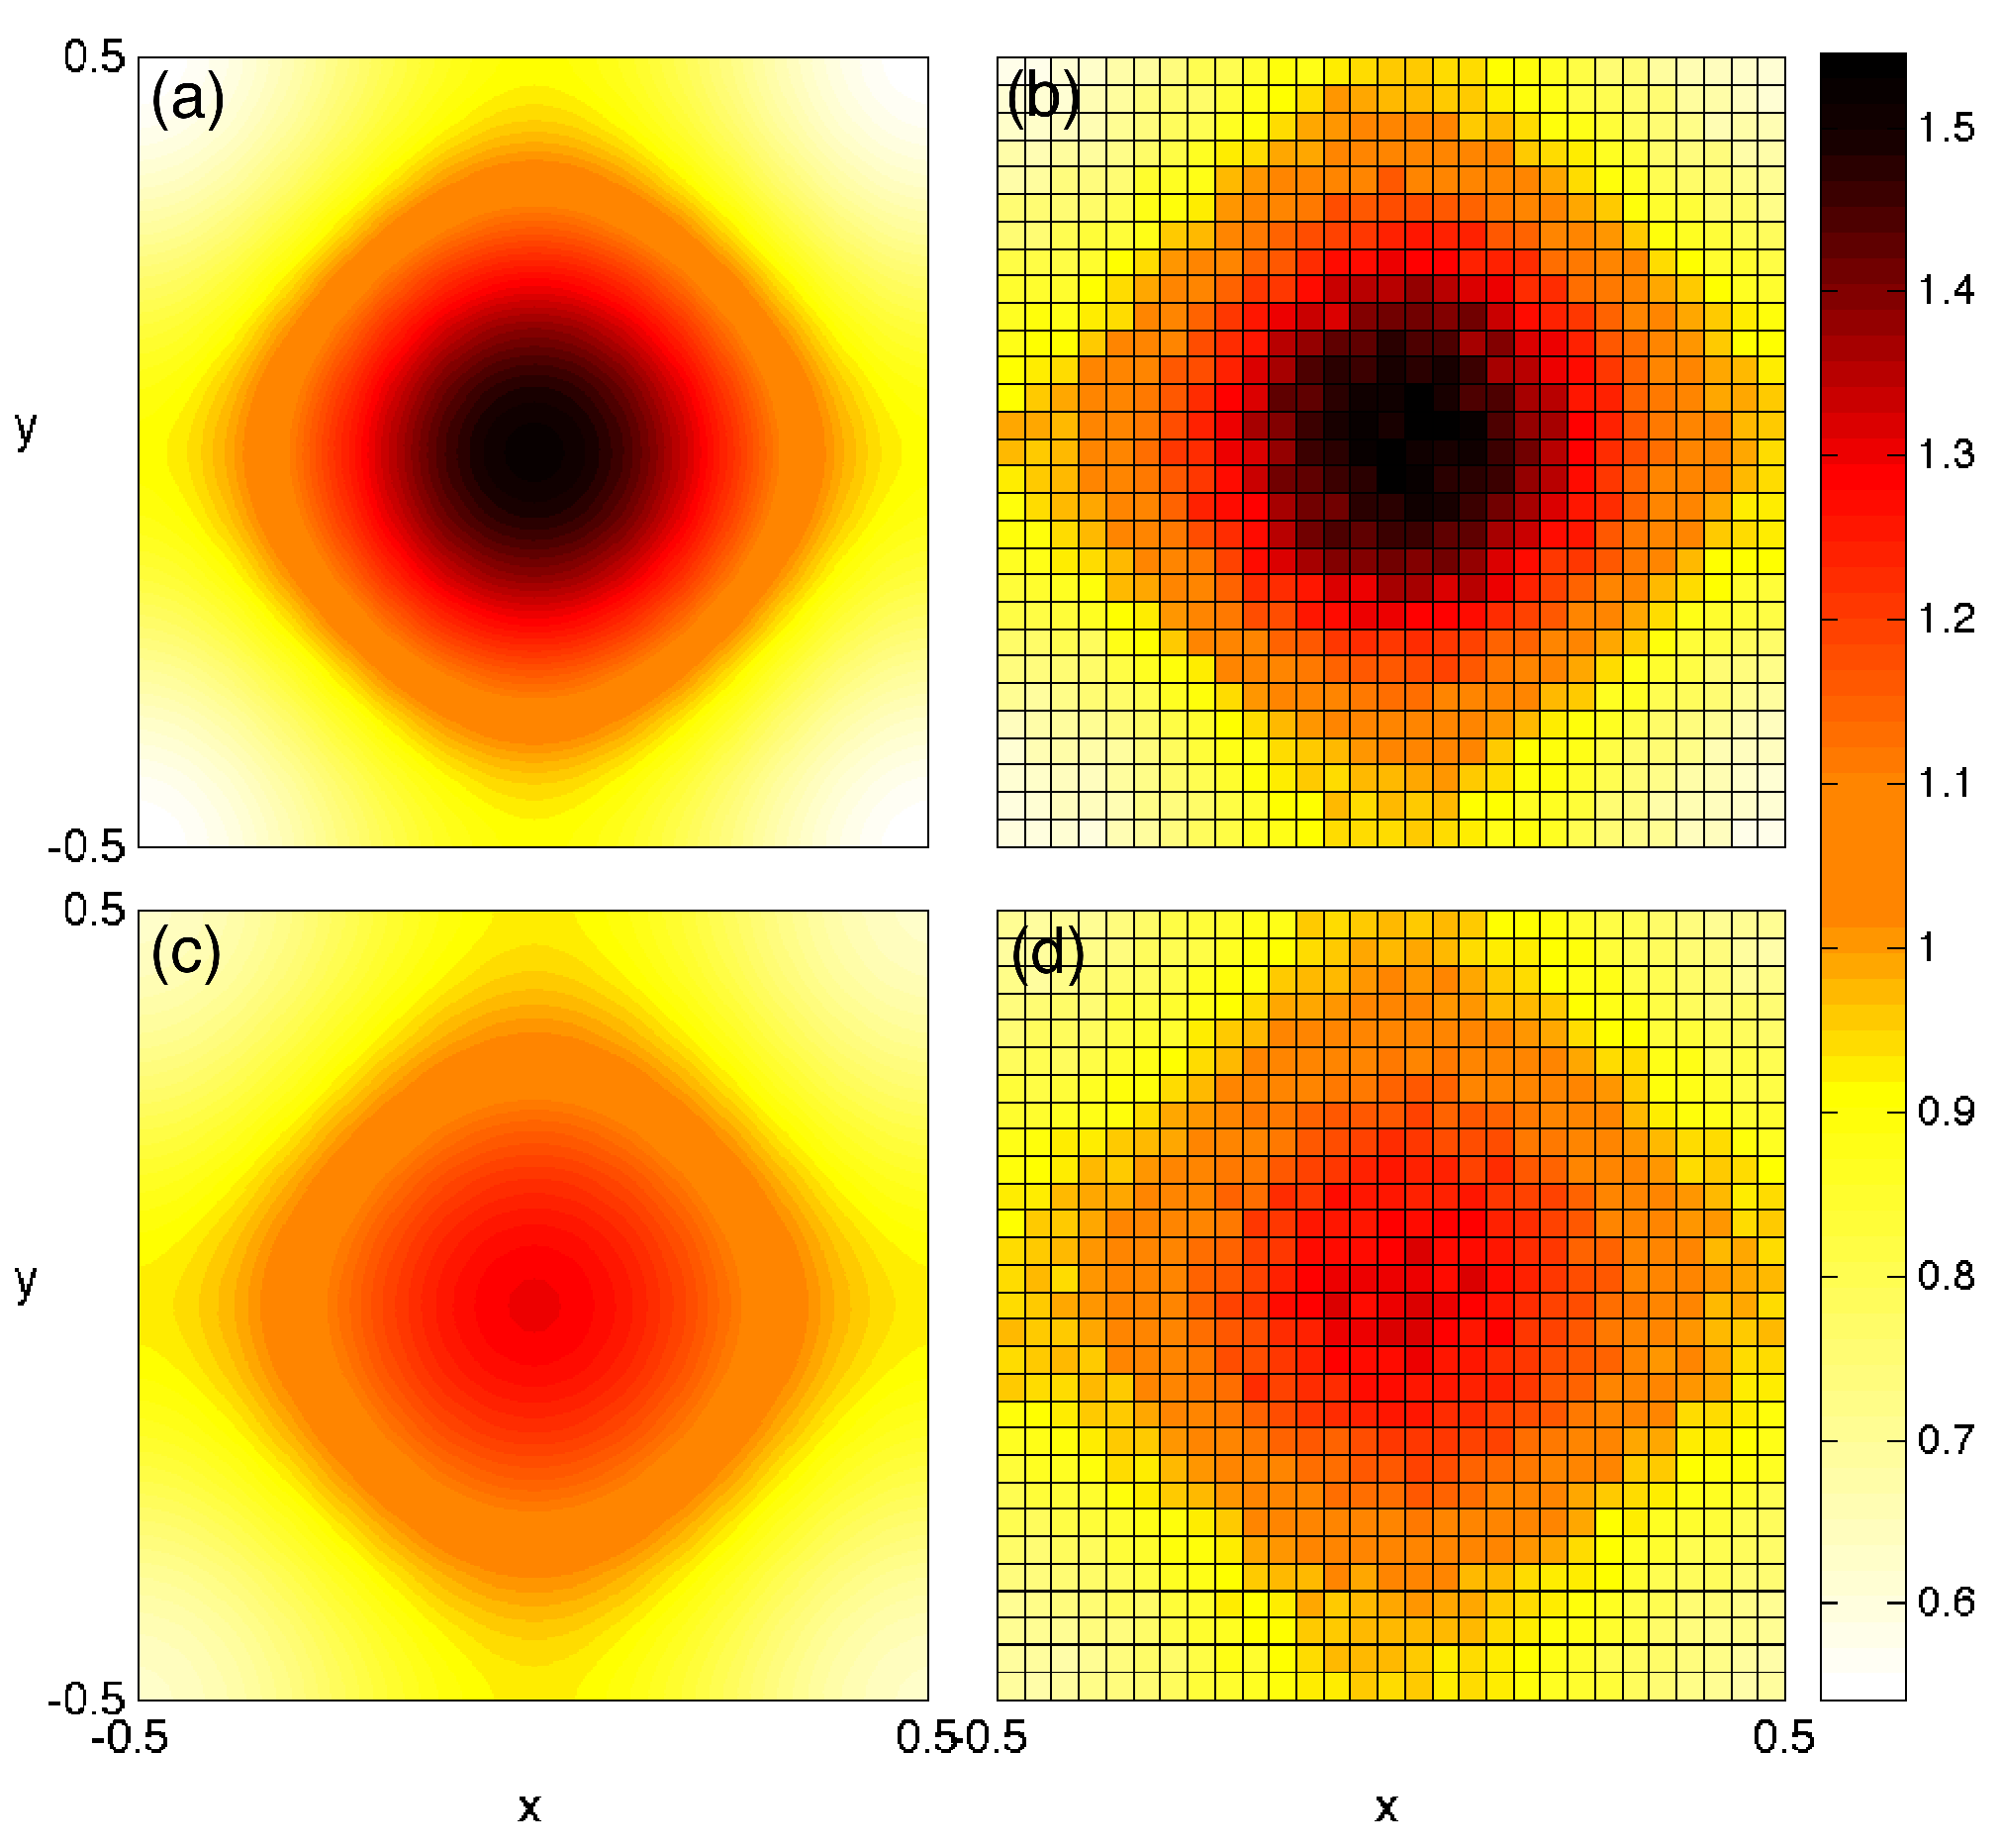
\includegraphics[width=0.8\textwidth]{intro/fig2_BC12.png}
    \caption{
    This figure from~\cite{Bruna2012} contains the following four plots, all of them are shown at time \( t=0.05 \). 
	For all plots, the initial condition is normally distributed with mean $(0,0)^T$ and standard deviation $0.09$. 
    (a) shows the solution of the linear diffusion Equation~\eqref{equ:pointparticle} for point particles. 
    (b) shows the histogram of a Monte Carlo simulation of the point particle model. 
    (c) shows the solution of the nonlinear diffusion Equation~\eqref{equ:hardsphere} for finite-sized particles. 
    (d) shows the histogram of a Monte Carlo simulation of the hard sphere model. 
    The Monte Carlo simulations used $10^4$ simulation runs each with a time step size of $10^-5$.
	We can see that the hard sphere model in (c) and (d) shows a quicker diffusion rate as the cell concentration in the centrum of the domain has already diffused more compared to the point particle model in (a) and (b). 
    }
    \label{fig:fig2BC12}
\end{figure}



% bachelor intro sp model 
\textbf{Soft sphere model} \\
Next, we consider an extension of the model by introducing deformable soft spherical particles. 
This new model incorporates the effect of deformation and interaction between particles through a potential energy function that depends on the distance between the particles.
The paper~\cite{Bruna2017}, written by Bruna, Chapman and Robinson, analyses the diffusion properties of such a model. \\
In contrast to the soft sphere model, the hard sphere model enforces rigid, non-deformable cell boundaries through reflective boundary conditions at a fixed separation distance, leading to abrupt, instantaneous collisions without any interface deformation. 
The soft sphere model uses a smoother approach including interaction potentials. \\
The equation of motion for each particle $i$ is given by
\begin{align*}
	d\vec{x}_i(t) = \sqrt{2D} \: dB_t^{(i)} + f(\vec{x}_i(t))\: dt - \sum\limits_{j\neq i} \nabla_{\vec{x}_i} u (\norm[ \vec{x}_i(t) - \vec{x}_j(t)]) \: dt, \qquad 1 \leq i \leq N_C,
\end{align*}
where $\nabla_{\vec{x}_i}$ is the gradient with respect to $\vec{x}_i$. \\
The effect of the interaction potential is to cause particles to repel or attract each other depending on the distance between them, rather than simply overlapping. \\
For the modeling of short range interacting soft sphere particles, the authors computed the one particle probability density $\rho(t, \vec{x})$ of finding a given particle at position $\vec{x}$ at time $t$ developing according to
\begin{align}
	\dfrac{\partial \rho}{\partial t} = \nabla_{\vec{x}} \cdot (D \nabla_{\vec{x}} \rho - f(\vec{x}) \rho + \alpha_u \epsilon_u^2(N_C-1)\rho \nabla_{\vec{x}} \rho)
	\label{equ:softsphere}
\end{align}
where $\alpha_u$ depends on the interaction potential $u$ and $0 < \epsilon_u \ll 1$ is the interaction range of $u$.
When comparing the first marginals of the soft sphere model Equation~\eqref{equ:softsphere} and the hard sphere model Equation~\eqref{equ:hardsphere}, we can see that they are similar in structure, with the main difference being the coefficients of the nonlinear diffusion terms. 
We can not clearly say which model diffuses faster, as this is dependent on the modelling of the soft interaction. \\
The influence of the cell hardness to the diffusion rate of the cell system will be investigated in this thesis. 
We even introduce a parameter that can continuously change the cell hardness from hard to soft. \\
While these models are powerful, they are limited to spherical particles and do not account for the complex shapes and deformations observed in biological cells.  \\



% phase field model
\textbf{Phase field model} \\
A new cell modeling framework is now considered. 
The phase field approach exhibits conceptual parallels with the soft sphere model proposed by Bruna, Chapman, and Robinson~\cite{Bruna2017}, particularly in how cell-cell interactions are modeled through a continuous repulsive energy that prevents overlap. \\
In both formulations, interactions are governed by a smooth, short range influence. 
The soft-sphere model derives its interaction dynamics from the potential energy $u(\|\vec{x}_i - \vec{x}_j\|_2)$, which leads to a nonlinear diffusion equation featuring a diffusion coefficient that depends on local density. \\
The phase field model resolves cell overlaps through a free energy producing a repulsive force between cells that scales with the local concentration of $\phi_i$. 
This enables gradual, continuous deformation of cell interfaces, thereby avoiding discontinuities in the dynamics that are characteristic of discrete collision models. 
Thus, the interaction mechanisms operate continuously and locally, ensuring a seamless transition between overlapping and non overlapping configurations while maintaining physical consistency in both models. \\
Nevertheless, the phase field model diverges fundamentally in its underlying structure: it is a continuum model based on partial differential equations that explicitly encodes cell morphology and internal organisation through the phase field variable $\phi_i$, enabling dynamic shape changes, topological transitions, and coupling to geometric features such as surface curvature. \\
The free energy functional encodes shape regularization, intercellular interactions, and physical constraints of the system. 
Unlike the soft-sphere model, which treats cells as point-like entities interacting via a smooth potential, the phase field model represents cells as much more complex, spatially extended, continuously structured entities, with their internal state fully described by the evolution of the phase field variable $\phi_i$. 
This enables a natural description of complex cell morphologies, topological transitions such as cell division or fusion, and the integration of cell mechanics with geometric curvature via extrinsic curvature contributions in the free energy. \\
Phase field variables represent cells as smooth functions $\phi_i(\vec{x}, t) \in [-1, 1]$, with $\phi_i > 0$ in the cell interior and $\phi_i <0$ in the exterior. 
The cell wall is denoted by values of $\phi_i = 0$. 
An illustration of a phase field variable is shown in Figure~\ref{fig:phasefield}. \\
\begin{figure}[h!]
	\centering
	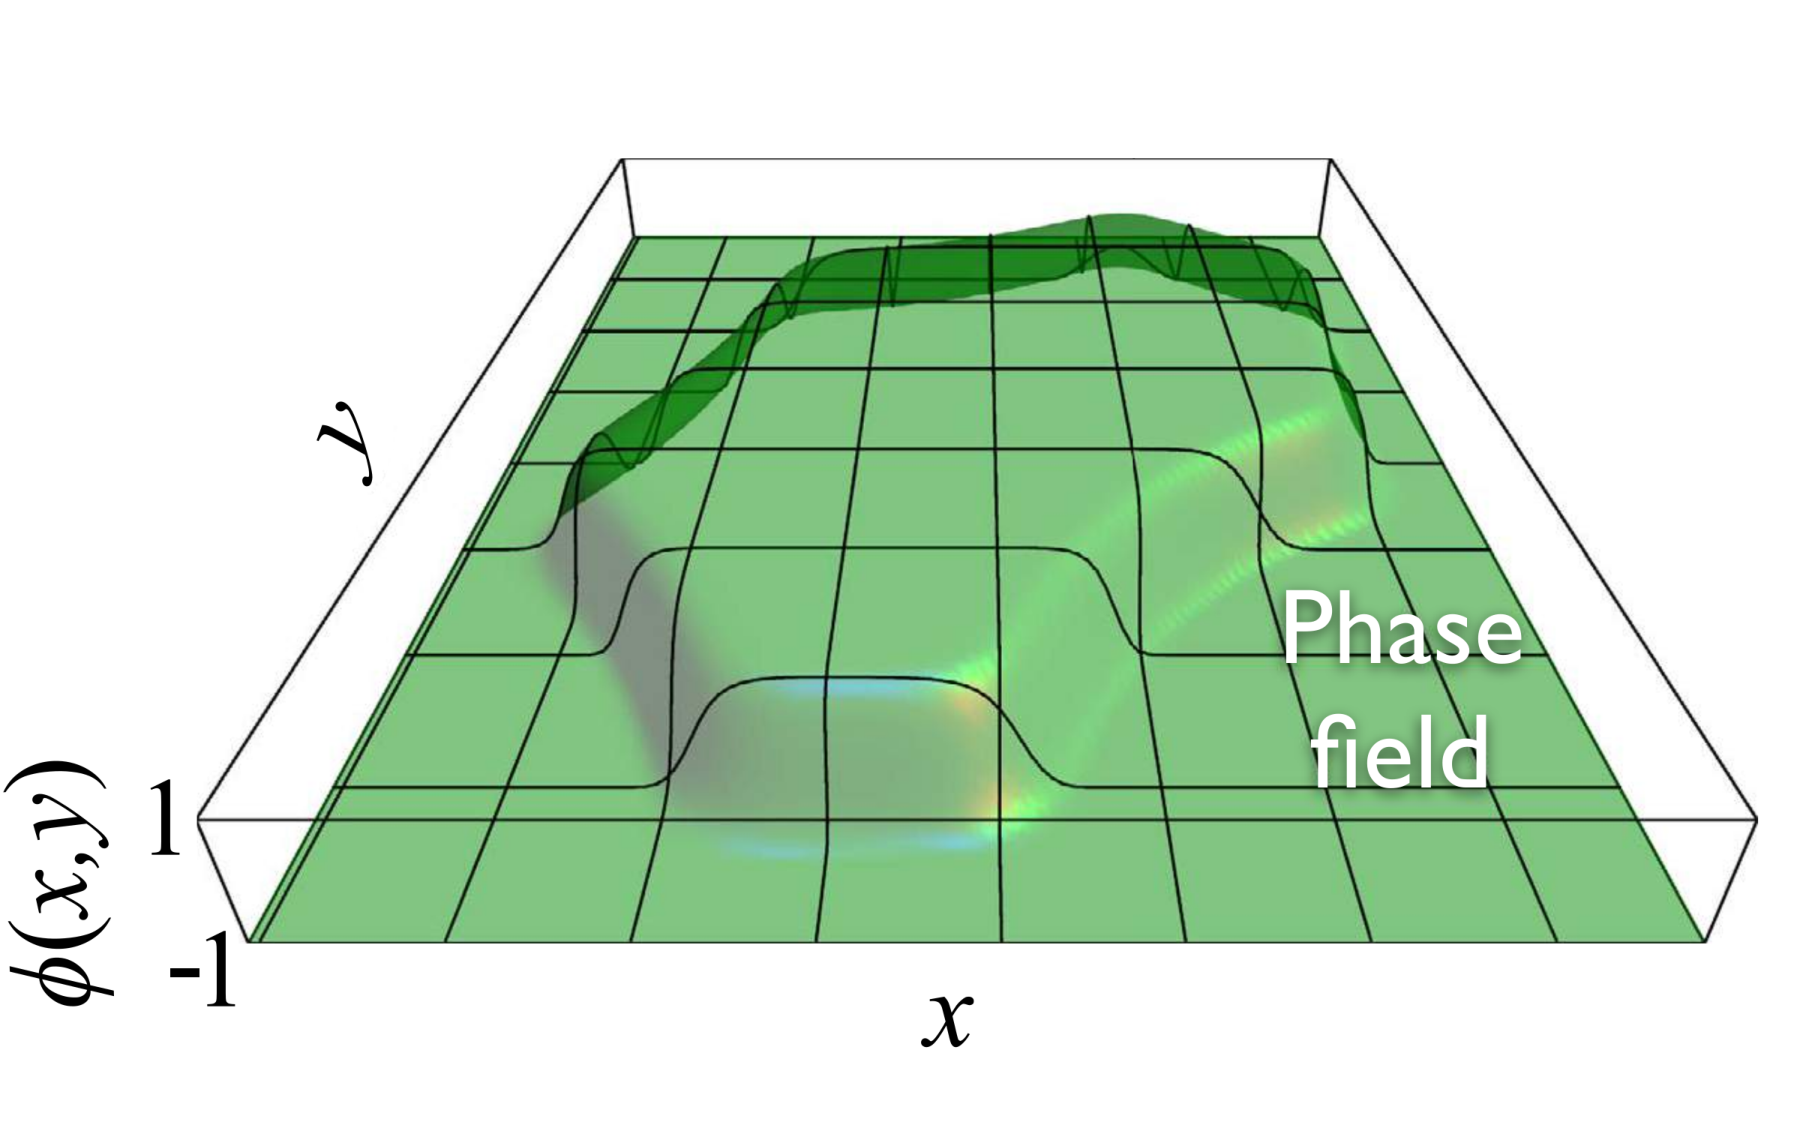
\includegraphics[width=0.8\textwidth]{intro/phasefield.pdf}
	\caption{A snapshot from the paper~\cite{alert2020} illustrating a phase field variable. 
	The cell's inside has value $\phi = 1$ and the outside $\phi = -1$. 
	}
	\label{fig:phasefield}
\end{figure}

%%% TODO: continue: 
The dynamics of a phase field variable $\phi_i$ can typically be given by a gradient flow of a free energy functional:
\begin{align*}
	\frac{\partial \phi_i}{\partial t} + v_0 (\vec{v}_i \cdot \nabla_{\vec{x}} \phi_i) = \Delta_{\vec{x}} \frac{\delta F}{\delta \phi_i}, \qquad 1 \leq i \leq N_C 
\end{align*}
where $\vec{v}_i$ is a vector field used to incorporate activity, with a self propulsion strength $v_0$, $F$ is a free energy, and $\dfrac{\delta F}{\delta \phi_i}$ denotes the first variation.\\
The free energy $F$ arises from a sum of different energies, 
\begin{align*}
	F = F_{CH} + F_{INT} + F_{M}. \\
\end{align*}
The first energy is a Cahn-Hilliard energy and could look like in~\cite{wenzel2021}
\begin{align*} 
	F_{CH} = \sum\limits_{i=1}^N \int_{\Omega} \dfrac{1}{Ca} \left( \dfrac{\epsilon}{2} \norm[\nabla_{\vec{x}} \phi_i]^2 + \dfrac{1}{\epsilon} W(\phi_i) \right) d\vec{x},
\end{align*}
where $\epsilon$ is a small parameter related to the interface thickness, and $Ca$ is a capillary number that scales the relative importance of surface tension.
The term $\norm[\nabla_{\vec{x}} \phi_i]^2$ penalises a long cell wall, as $\nabla_{\vec{x}} \phi_i \neq 0$ only at the cell wall.
Thus, the Cahn-Hilliard energy always tries to minimize the area of the cell interface. \\
$W(\phi_i) = \dfrac{1}{4} (\phi_i^2 - 1)^2$ is a double-well potential. 
This energy ensures that each $\phi_i$ maintains a stable interface of $[-1,1]$.  \\ 
The second energy term $F_{INT}$ models cell-cell interactions and could be defined as in~\cite{wenzel2021}
\begin{align*}
	F_{INT} = \sum\limits_{i=1}^N \frac{1}{Ca} \int_{\Omega} B(\phi_i) \sum\limits_{j \neq i} w(d_j) \: d\vec{x},
\end{align*}
where 
\[B(\phi_i) = \dfrac{3}{4\sqrt{2}\epsilon} (\phi_i^2 - 1)^2\]
is an approximation of the delta function of the cell boundary that is non-zero only at the cell wall.
The sum in the integral accounts for the interaction with all other cells $j \neq i$ through a short-range potential $w(d_j)$, where $d_j$ is the signed distance function to the cell boundary of cell $j$.  
When employing this dynamics, the interaction force $F_{INT}$, acts to reduce or eliminate cell overlaps. \\
The third energy term $F_M$ differs for different models and incorporates additional mechanical properties of the cells, such as area conservation or bending energy.
This energy is dependent on the use case of the model. \\
It can have a big influence on the dynamic of a phase field model, as analysed in~\cite{wenzel2021}, where the authors focussed on the influence of microscopic details to incorporate active forces on emerging phenomena.\\
Four different approaches are considered.
One in which the activity is determined by a random orientation, one where the activity is related to the deformation of the cells, and two models with subcellular details to resolve the mechanochemical interactions underlying cell migration. \\
The random model determines the direction of motion on the single cell level by a stochastic process. 
The second model is called elongation model.
It identifies the longest axis of the cell's phase field and aligns the direction of motion with this axis. \\
The third and fourth models presented are referred to as the polar model and the nematic model, respectively.
Cell motion strength and direction are determined based on subcellular details at the single-cell level. \\
All models are compared with respect to generic features, such as coordination number distribution, cell shape variability, emerging nematic properties, as well as vorticity correlations and flow patterns in large confluent monolayers and confinements. 
We can see the results in Table~\ref{table:phasefield}. \\

\begin{table*}[h!]
	\centering
	\begin{tabular}{>{\small}l >{\small}c  >{\small}c  >{\small}c  >{\small}c} % l = left aligned, c = centered, r = right aligned
	\hline
	characteristic & Random & Elongation & Polar & Nematic \\ 
	\midrule
	Coordination number distribution & ($\checkmark$) & ($\checkmark$) & ($\checkmark$) & ($\checkmark$) \\
	& & & &  \\
	
	Shape variability & ($\checkmark$) & $\checkmark$ & $\checkmark$ & ($\checkmark$) \\
	& & & &  \\
	
	Rosette ratio & \multicolumn{4}{>{\small}c}{Differences between models} \\
	& & & &  \\

	Velocity distribution of  & \multicolumn{4}{>{\small}c}{Differences between models} \\
	topological defects  & & & &  \\
	& & & &  \\

	Correlation between direction of  & \Large $\boldsymbol{\times}$ & $\checkmark$ & $\checkmark$ & ($\checkmark$) \\
	motion and orientation of defect  & & & &  \\
	& & & &  \\

	Elastic property of + 12 defect & \Large $\boldsymbol{\times}$ & Extensile & Contractile & Contractile \\
	& & & &  \\
	
	Active turbulence & ($\checkmark$) & ($\checkmark$) & ($\checkmark$) & ($\checkmark$) \\
	& & & &  \\
	
	Vorticity-vorticity correlation & \multicolumn{4}{>{\small}c}{Similar for all models} \\
	& & & &  \\

	Dependency of defect  & Linear & Linear & Linear & Constant \\
	density on activity  & & & &  \\
	& & & &  \\

	Rotational motion in  & \Large $\boldsymbol{\times}$ & ($\checkmark$) & \Large $\boldsymbol{\times}$ & \Large $\boldsymbol{\times}$ \\
	circular confinement  & & & &  \\

	\bottomrule
	\end{tabular}
	\caption{Comparison of the four different phase field models from~\cite{wenzel2021} with respect to various characteristics observed in experiments. 
	A check mark $\checkmark$ indicates observed agreement, $\mathnormal{\Large \boldsymbol{\times}}$  
	indicates disagreement and ($\checkmark$) indicates only qualitative agreement with universal feature. 
	If experimental data are not available or insufficient for a comparison, only similarities or differences of the models are noted.}
	\label{table:phasefield}
\end{table*}

The goal of this paper is a systematic comparison of these approaches and their linkage with statistical observables of experiments to provide a route towards predictive simulations of patterns and correlations in cell colonies. 
Model predictions are compared with experimental data from various cell cultures. 
The qualitative differences observed highlight the importance of microscopic details. \\ 
\begin{figure}[h!]
	\centering
	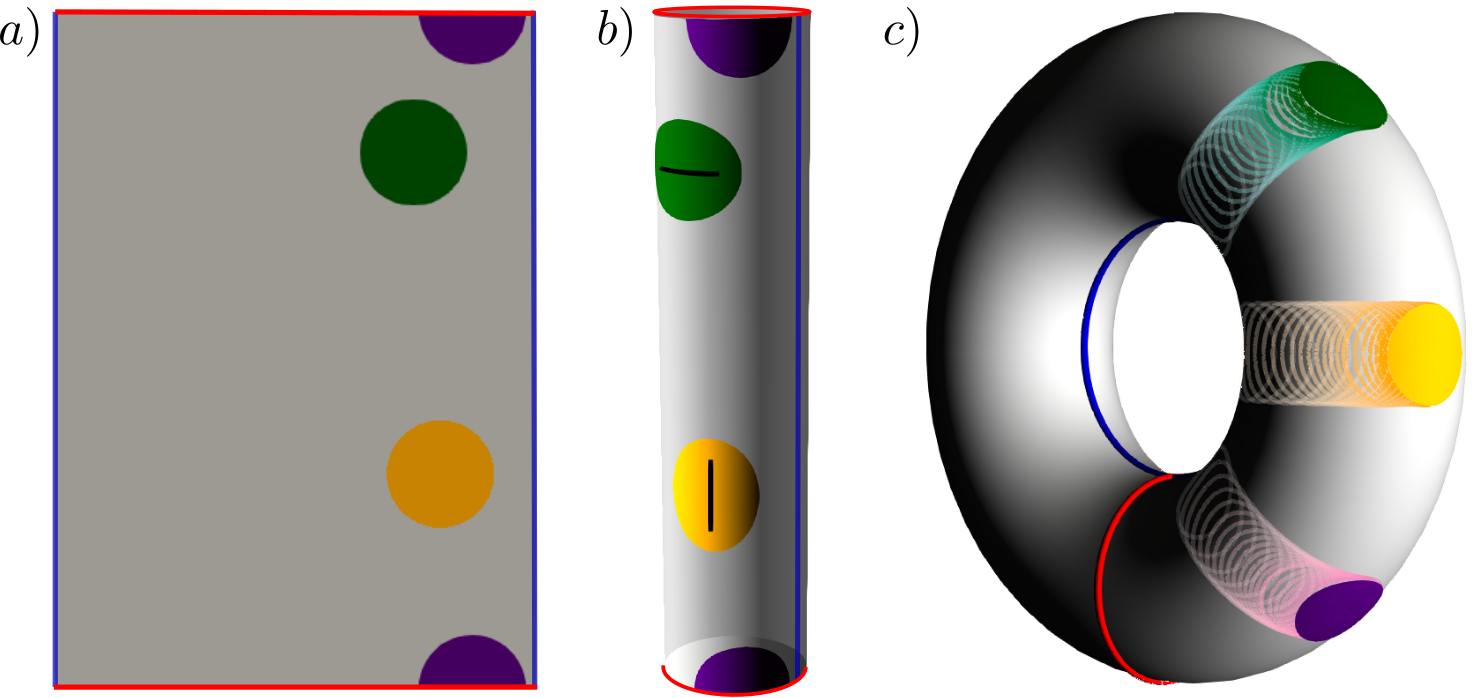
\includegraphics[width=0.8\textwidth]{intro/curved_phasefield.png}
	\caption{A figure from the paper~\cite{Happel2023} showing a phase field variable $\phi$ on a curved domain, specifically a torus. 
	In (a) and (b), the surface of the torus from (c) is shown as a parametrization on a rectangle, where the blue edges are identified (glued together) to form the toroidal direction, and the red edges are similarly identified to form the poloidal direction. 
	Red and blue lines represent periodic boundary conditions, which are enforced by gluing the corresponding edges in (b) and (c).
	The color coding corresponds to the extrinsic curvature parameter $E_c$ (see Eq.~(3)): $E_c = 0$ (purple) results in a geodesic circle on both geometries; $E_c > 0$ (green) favors alignment with the direction of maximum absolute curvature; $E_c < 0$ (yellow) favors alignment with the direction of minimal absolute curvature. 
	Cell elongation is highlighted for visibility. 
	On toroidal surfaces, cell shape depends on position due to varying curvature. 
	(c) shows the trajectories, final positions, and shapes of cells over time. 
	The influence of extrinsic curvature is not apparent in the final configuration, as all shapes were obtained by solving Eq.~(1) with $v_0 = 0$. 
	}
	\label{fig:curved_phasefield}
\end{figure}
A related study by Happel and Voigt~\cite{Happel2023} employs phase field models to investigate cell dynamics, specifically focusing on the influence of curved domains (defined as tori) on collective cell behavior. 
The visualization of cells on a torus is shown in Figure~\ref{fig:curved_phasefield}. \\ 
Their work examines emergent phenomena like coordinated rotation on curved surfaces, driven by curvature alignment and self-propulsion. 
Unlike the soft-sphere model, which typically assumes spherical symmetry and isotropic interactions, the phase field approach allows for the incorporation of anisotropic effects, such as alignment with principal curvature directions, through geometric coupling terms. 
This capability enables the simulation of complex collective behaviors but also increases computational demands compared to simpler point-particle models. \\
The phase field model developed by Happel and Voigt~\cite{Happel2023} highlights the critical role of extrinsic curvature coupling in dictating the alignment of cell elongation with principal curvature directions and the emergence of coordinated rotation in epithelial layers on curved surfaces. 
By combining a diffuse interface representation with a free energy incorporating both intrinsic and extrinsic geometric terms, their simulations successfully reproduce key experimental observations, including spontaneous rotation on cylindrical surfaces and curvature-dependent morphological changes on tori. 
This work emphasizes the significance of geometric constraints in tissue morphogenesis and offers a framework for investigating how curvature influences collective cell dynamics beyond planar environments. \\



\textbf{Vertex model} \\
The last cell model approach is also the approach we choose in this thesis. 
Vertex models represent a powerful and versatile approach for simulating the mechanical behavior of biological cells and tissues. \\
Originating from materials science and solid mechanics, these models represent cells as polygons, where the boundaries are defined by a discrete set of vertices connected by edges. 
The degrees of freedom in these models are precisely these vertices, meaning that all the cell model dynamics are applied only to the vertices. \\
The cell dynamic in a vertex model is usually given by the equation
\begin{align}
	\dfrac{d \vec{x}_i}{dt} = F_i^m, \label{eq:vertexmodel}, 
\end{align}
where $F_i^m$ is the total force acting on vertex $1 \leq i \leq N_V$ of cell $1 \leq m \leq N_C$. \\
Like in the phase field model, $F_i^m$ is a sum of different forces that define the cell behavior, such as the cell flexibility or the interaction with other cells. 
The forces participating in $F_i^m$ or often found as negative gradients of energies that shall be minimized. 
This method called gradient flow is also used for phase field models. \\
Due to their discrete nature, vertex models are computationally efficient compared to continuum models, while still providing rich insights into the interplay between cell mechanics and collective behavior, making them invaluable for understanding fundamental principles governing cell organization and tissue dynamics across diverse biological contexts. \\
This geometric representation allows for the incorporation of key cellular properties, such as surface tension, cortical tension, adhesion, and local shape constraints, into an energy functional. 
Minimizing this energy through computational simulation enables the capture of emergent phenomena like tissue morphogenesis, cell migration, wound healing, and pattern formation. \\

% fletcher 
The paper \cite{Fletcher14} developed a sophisticated vertex based model to simulate the dynamic behavior of confluent epithelial cell sheets, representing tissues where cells completely cover the available space without gaps. 
Their model aims to capture key biological processes observed in real epithelial tissues. \\
Conservation of cell area and perimeter ensures cells maintain their size and shape during deformation.
Junctional rearrangements, including neighbor exchange and vertex/edge merging, enable cell migration and tissue remodeling.
Cell division is modeled by creating a rosette structure from multiple adjacent vertices and cell growth and death simulate changes in individual cell size.
A detailed exploration of the implementation and specific consequences of these confluent specific mechanics is beyond the scope of this work.
While these mechanisms are essential for understanding the complex dynamics of confluent tissues, the focus of this thesis lies on non confluent cell models, where the presence of interstitial space and variable packing density leads to distinct physical behaviors. \\

% jamming (deformable particles in confluent model)
Boromand, Merkel, and Manning~\cite{Boromand2018} investigated the jamming transition in a system of deformable cells using a vertex model. 
Of particular interest is their development of a non confluent cell model meaning that gaps between the cells are allowed by the model. 
This model is versatile and can be applied to simulate cells, foams, emulsions, and other soft particulate materials. \\
It uniquely combines the ability to represent individual deformable particles with the established shape energy function of the vertex model. 
This shape energy function incorporates terms that penalize deviations from a target area ($a$) and perimeter ($p$), along with repulsive interparticle forces to prevent overlap. \\
The model defines polygons with $N_V \in \N$ vertices, where the bond vector $\vec{l}_{mi}$ connects vertex $\vec{v}_{m,i}$ to $\vec{v}_{m,i+1}$, i.e. vertex $i$ to vertex $i+1$ of cell $m$.
The complete shape energy function, which governs the particle dynamics, integrates these various contributions:
\begin{align*}
	U &= U_{\text{contract}} + U_{\text{compress}} + U_{\text{line tension}} + U_{\text{bending}} + U_{\text{interaction}}.
\end{align*}

The first energy reads
\begin{align*}
	U_{\text{contract}} &= \frac{k_l N_V}{2} \sum\limits_{m=1}^{N_C} \sum\limits_{i=1}^{N_V} (l_{m,i}-l_0)^2,
\end{align*}
where $k_l$ is the spring constant and $l_0$ is the equilibrium length of the edges. 
It penalises contractions or expansion of cell edges and makes the edges return to their desired length $l_0$. \\ 
Similarly, the second force $U_{\text{compress}}$ stabilises the cells area to a equilibrium area $a_0$ 
\begin{align*}
	U_{\text{compress}} &= \frac{k_a}{2} \sum\limits_{m=1}^{N_C} (a_m - a_0)^2, 
\end{align*}
where $k_a$ is compressibility constant. \\ 
The line tension energy is another energy working with the cell edges.
It sanctions long edges with the formula 
\begin{align*}
	U_{\text{line tension}} &= \gamma \sum\limits_{m=1}^{N_C} \sum\limits_{i=1}^{N_V} l_{m,i} ,
\end{align*}
where $\gamma$ is the line tension coefficient. \\
The last shape energy is given by the bending energy. 
It acts to resist changes in the angles between adjacent edges of the polygonal cells.
This energy encourages the cells to maintain smooth, relatively straight boundaries and discourages sharp bends or kinks.
\begin{align*}
	U_{\text{bending}} &= \frac{k_b}{2 N_V} \sum\limits_{m=1}^{N_C} \sum\limits_{i=1}^{N_V} \left( \frac{2( \hat{l}_{m,i} - \hat{l}_{m,i+1})}{l_{m,i} - l_{m,i+1}}  \right)^2 ,
\end{align*}
where $k_b$ is the bending rigidity constant, $\hat{l}_{m,i} = \frac{\vec{l}_{m,i}}{\norm[\vec{l}_{m,i}]} $ is the unit vector of $\vec{l}_{m,i}$.
These four energies are conserving a specific cell shape. \\
\begin{figure}[h!]
	\centering
	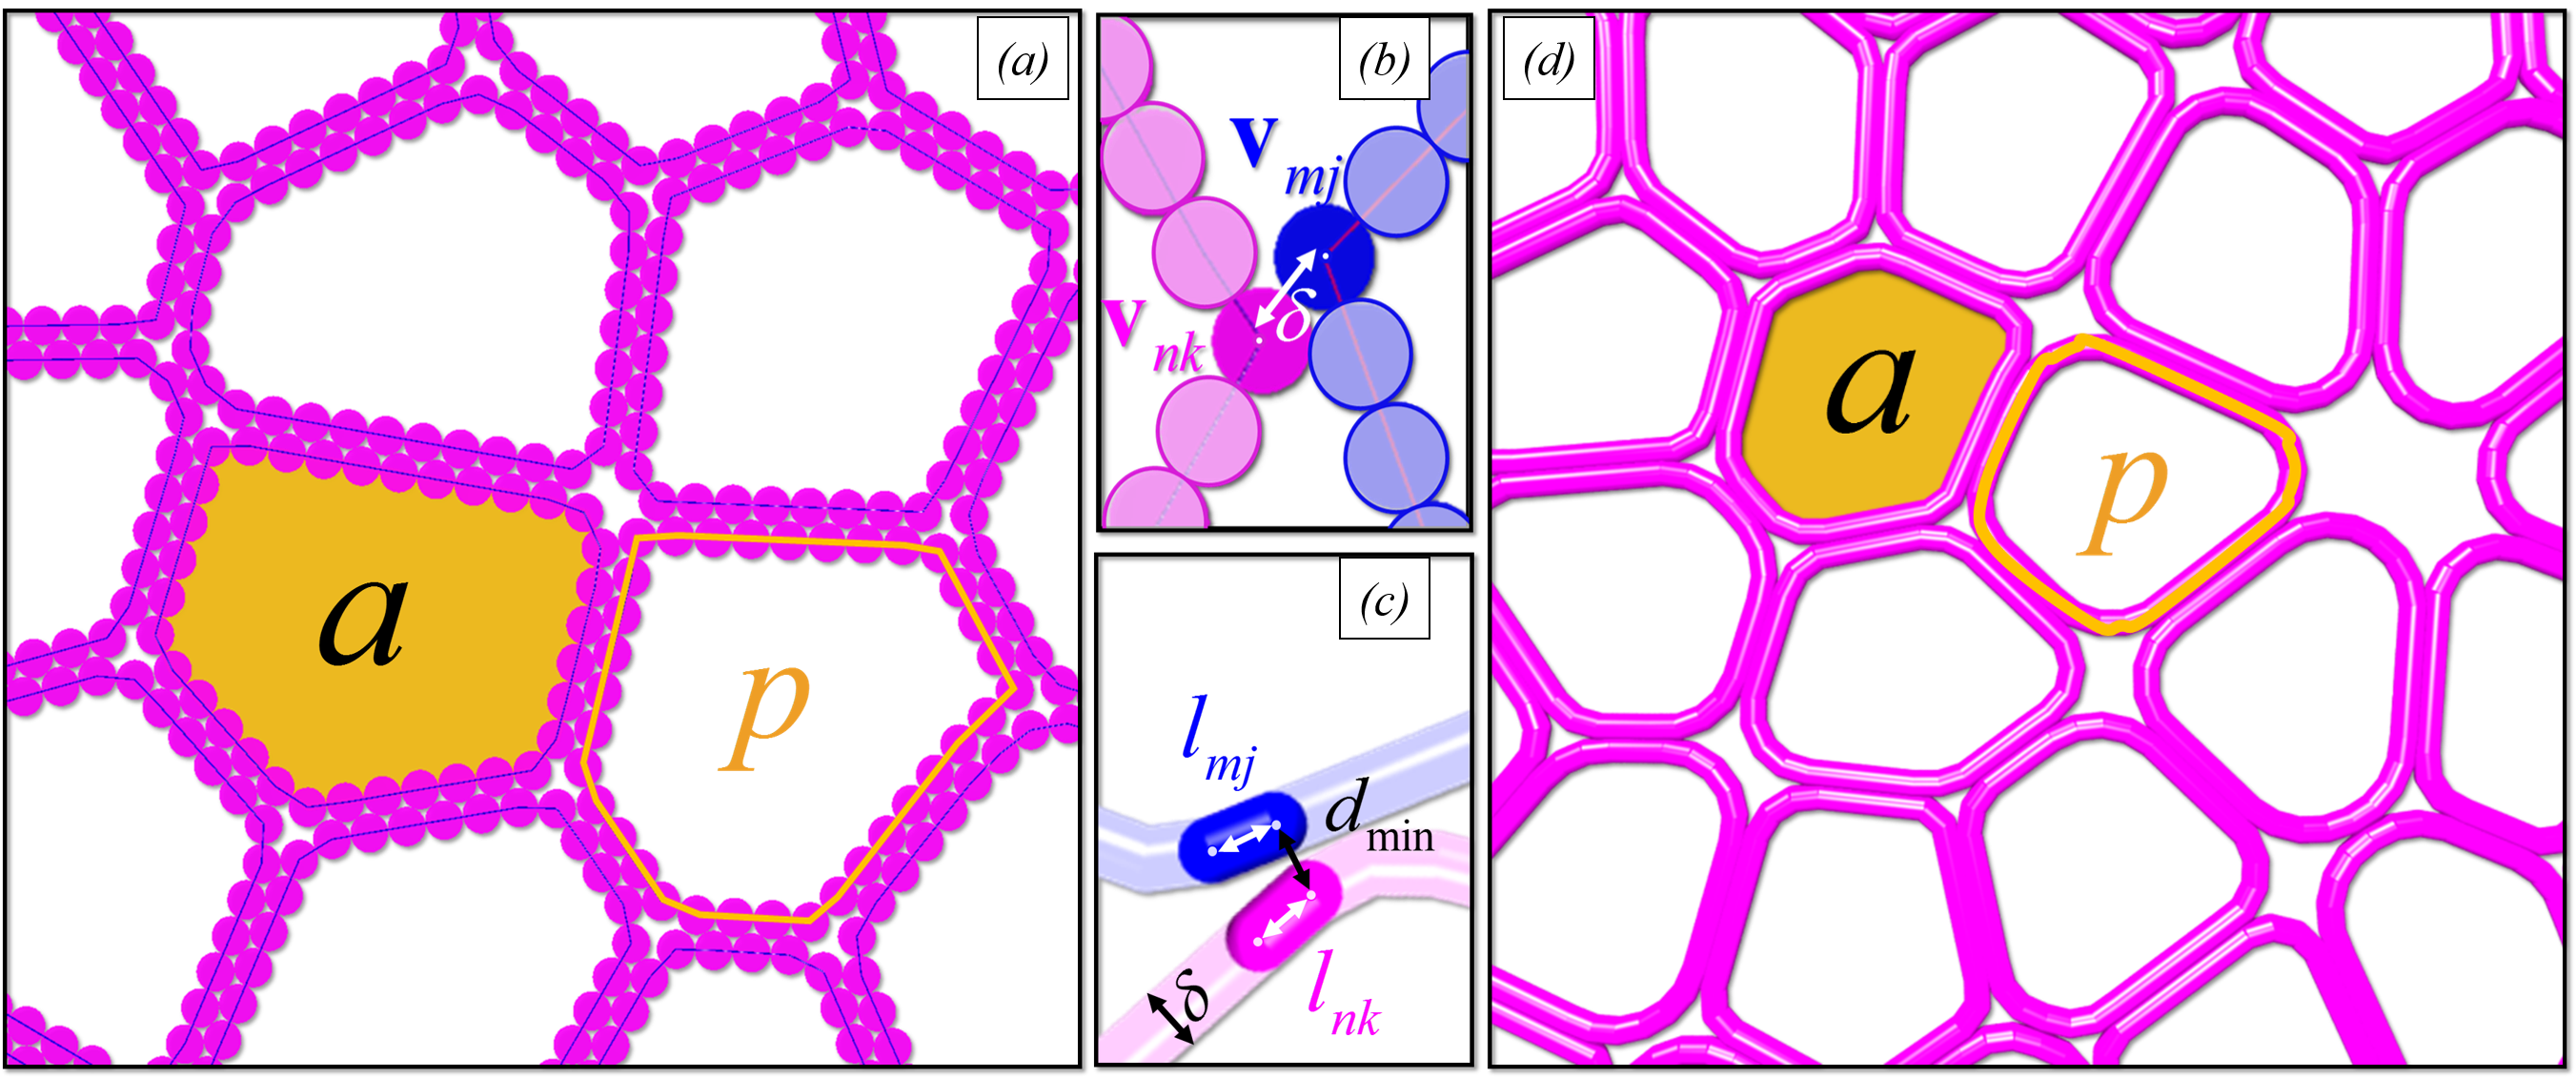
\includegraphics[width=0.8\textwidth]{intro/jamming.png}
	\caption{A snapshot from the paper~\cite{Boromand2018} illustrating a configuration of vertex-based deformable cells. 
	Schematic of deformable polygons with $N_V = 34$ vertices (where the position of the $j$-th vertex in the $m$-th polygon is denoted by $\vec{v}_{m,j}$), area $a_m$, and perimeter $p_m$. 
	The edge $l_{m,j} = p_m / N_V$ represents the line segment connecting vertices $j$ and $j+1$ in polygon $m$. 
	Two methods are used to model the edges of deformable polygons: (a) and (b) show the RS method, where disks of diameter $\delta$ are centered at the polygon vertices; (c) and (d) show the SS method, where polygon edges are modeled as circulo-lines of width $\delta$. 
	The quantity $d_{\text{min}}$ denotes the minimum distance between the line segments $l_{m,j}$ and $l_{n,k}$.
	}
	\label{fig:vertex}
\end{figure}
There are two different methods to model the repulsive interaction between two deformable polygons called rough surface (RS) and smooth surface (SS) method.
Both methods are illustrated in Figure~\ref{fig:vertex}. \\ 
In the Rough Surface (RS) method, the discrete nature of the polygonal cell representation is emphasized. 
Each vertex of a cell is treated as the center of a rigid disk with a fixed diameter, set to $\delta = l_0$ (equilibrium bond length).
Repulsive interactions between cells are then modeled as linear spring forces that arise when these disks overlap. 
This approach effectively simulates a rough surface interaction, characterized by discrete points of repulsion localized at the cell vertices, rather than a continuous interaction across the cell boundary.
\begin{align*}
	U_{\text{RS}} &=  \sum\limits_{m=1}^{N_C} \sum\limits_{n>m}^{N} \sum\limits_{j=1}^{N_V} \sum\limits_{k=1}^{N_V} \frac{k_r}{2} (\delta - |\vec{v}_{m,j} - \vec{v}_{n,k} |)^2 \times \Theta(\delta - |\vec{v}_{m,j} - \vec{v}_{n,k}) ,
\end{align*}
where $k_r$ is the repulsive constant and $\Theta$ is the Heaviside step function, that is either $1$ for a positive argument or $0$ otherwise. \\
In contrast to the RS method, the Smooth Surface (SS) method adopts a smoother representation, modeling polygon edges as circulo-lines, essentially line segments with a finite width $\delta$. 
Repulsive forces are then calculated based on the minimum distance $d_{\text{min}}$, between these circulo-line segments belonging to different polygons. 
The interaction energy is then formulated using this minimum distance $d_{\text{min}}$.
\begin{align*}
	U_{\text{SS}} = \sum_{m=1}^{N_C} \sum_{n \neq m} \sum_{j=1}^{N_V} \sum_{k=1}^{N_V} \frac{1}{2} k_r \left( \delta - d_{\min} \right)^2 \Theta\left( \delta - d_{\min} \right).
\end{align*}
This method provides a smoother, more continuous repulsion, better approximating the behavior of soft, continuous interfaces. \\ 
Despite the different interaction mechanisms, both methods yield similar structural and mechanical properties at jamming onset. 
This indicates that the overall jamming behavior is robust to the specific choice of interaction model. \\


% transition to our model:
\textbf{Discrete Form model} \\ 
% - The model developed in this thesis is called discrete form (DF) model
% - In this thesis, we derive and study a non confluent DF model that systematically investigates how cellular deformability—controlled by the hardness parameter $h$—influences the overall diffusivity of the cell system. 
% - By connecting our model to the established frameworks of Bruna and Chapman~\cite{Bruna2012, Bruna2017} and Happel and Voigt~\cite{Happel2023}, we provide a unified perspective on cell dynamics that spans from rigid to deformable regimes.
% - our model is also vertex based like in~\cite{Fletcher14, Boromand2018} and we use it in a non confluent setting, like in~\cite{Boromand2018}
% - our model uses less vertices (usually $N_V=6$ for us, whereas $N_V=34$ in~\cite{Boromand2018})
% - shape preserving forces and interaction forces 
% - we use different energies: area, edge, interior angle energy for shape preservation and deforming overlap force and bounce overlap force for degenerating cell overlaps 
% - The dynamics for these energies are governed by gradient flows of energy functionals, ensuring that the system evolves toward lower-energy configurations. 
% - this ensures: we can use represent a wide range of desired cell shapes like in the discussed phase field and vertex models 
% - cell deformation is allowed like in~\cite{Boromand2018, Fletcher14,wenzel2021,Happel2023}
% - These shared principles provide a strong foundation for comparing our model to established frameworks.
% - we have introduced the shape preserving forces as well as the deforming overlap force in my bachelors thesis ~\cite{Vogel2023}, but here in the masters thesis, there were many bug fixes, parallelisation of the code, redefinition of forces now using neighboring vertices done to make to them in the sections~\ref{model, dynamics}, really enabling them to savely work stable in big simulations like the monte carlo simulations in chapter~\ref{sanitycheck}.
% - In this chapter we did a sanity check looking for recreate the diffusion dynamics for the point particle model and the hard spheres from \cite{Bruna2012}. 
% - we enable a transition from hard discs to soft discs with hardness parameter $h \in [0,1]$ 
% - overall 3 big monte carlo simulations were made in Chapter~\ref{sanitycheck} with different hardnesses $h \in {0,0.5,1}$ representing soft, mid and hard cells.  
% - Afterwards, we discuss the density dynamic in Chapter~\ref{density}.
% - In the end, we give a conclusion and an outlook on how this model could be used or extanded in the future.  
This thesis introduces the Discrete Form (DF) cell model, a vertex based framework inspired by~\cite{Fletcher14, Boromand2018} for simulating cell dynamics in non-confluent systems, similar to~\cite{Boromand2018}, but typically using fewer vertices (e.g., $N_V=6$). \\
The DF model incorporates shape preserving forces (area, edge, interior angle energies) and interaction forces (deforming and bounce overlap forces) derived as gradient flows of energy functionals, allowing for cell deformation like in~\cite{Boromand2018, Fletcher14,wenzel2021,Happel2023} and ensuring evolution towards lower-energy configurations. 
This allows representation of a wide range of desired cell shapes. \\
The core contribution of this thesis is a non confluent DF model that systematically investigates how cellular deformability, controlled by a hardness parameter $h \in [0,1]$, influences the overall diffusivity of the cell system, enabling a transition from hard disc-like to soft disc-like behavior. 
Building upon the foundations laid in the Bachelor's thesis~\cite{Vogel2023}, significant improvements were made, including bug fixes, code parallelization, and reformulation of forces for stable large-scale simulations (detailed in Sections~\ref{model} and~\ref{dynamics}). \\
Chapter~\ref{sanitycheck} presents a rigorous validation by recreating the diffusion dynamics of the point particle and hard sphere models from~\cite{Bruna2012} through extensive Monte Carlo simulations with varying hardness ($h \in \{0, 0.5, 1\}$), representing soft, intermediate, and hard cell behaviors. \\
Subsequently, Chapter~\ref{density} analyzes the resulting density dynamics. 
By connecting to the frameworks of~\cite{Bruna2012, Bruna2017, Boromand2018}, this work provides a unified perspective on cell dynamics spanning rigid to deformable regimes. 
Finally, the thesis concludes with a summary of findings and an outlook on potential future extensions and applications of the DF model.
